\documentclass[margin=5mm]{standalone}
\usepackage{tikz}
\usepackage{array}
\usetikzlibrary{positioning, arrows.meta, calc, shapes.geometric}

\begin{document}
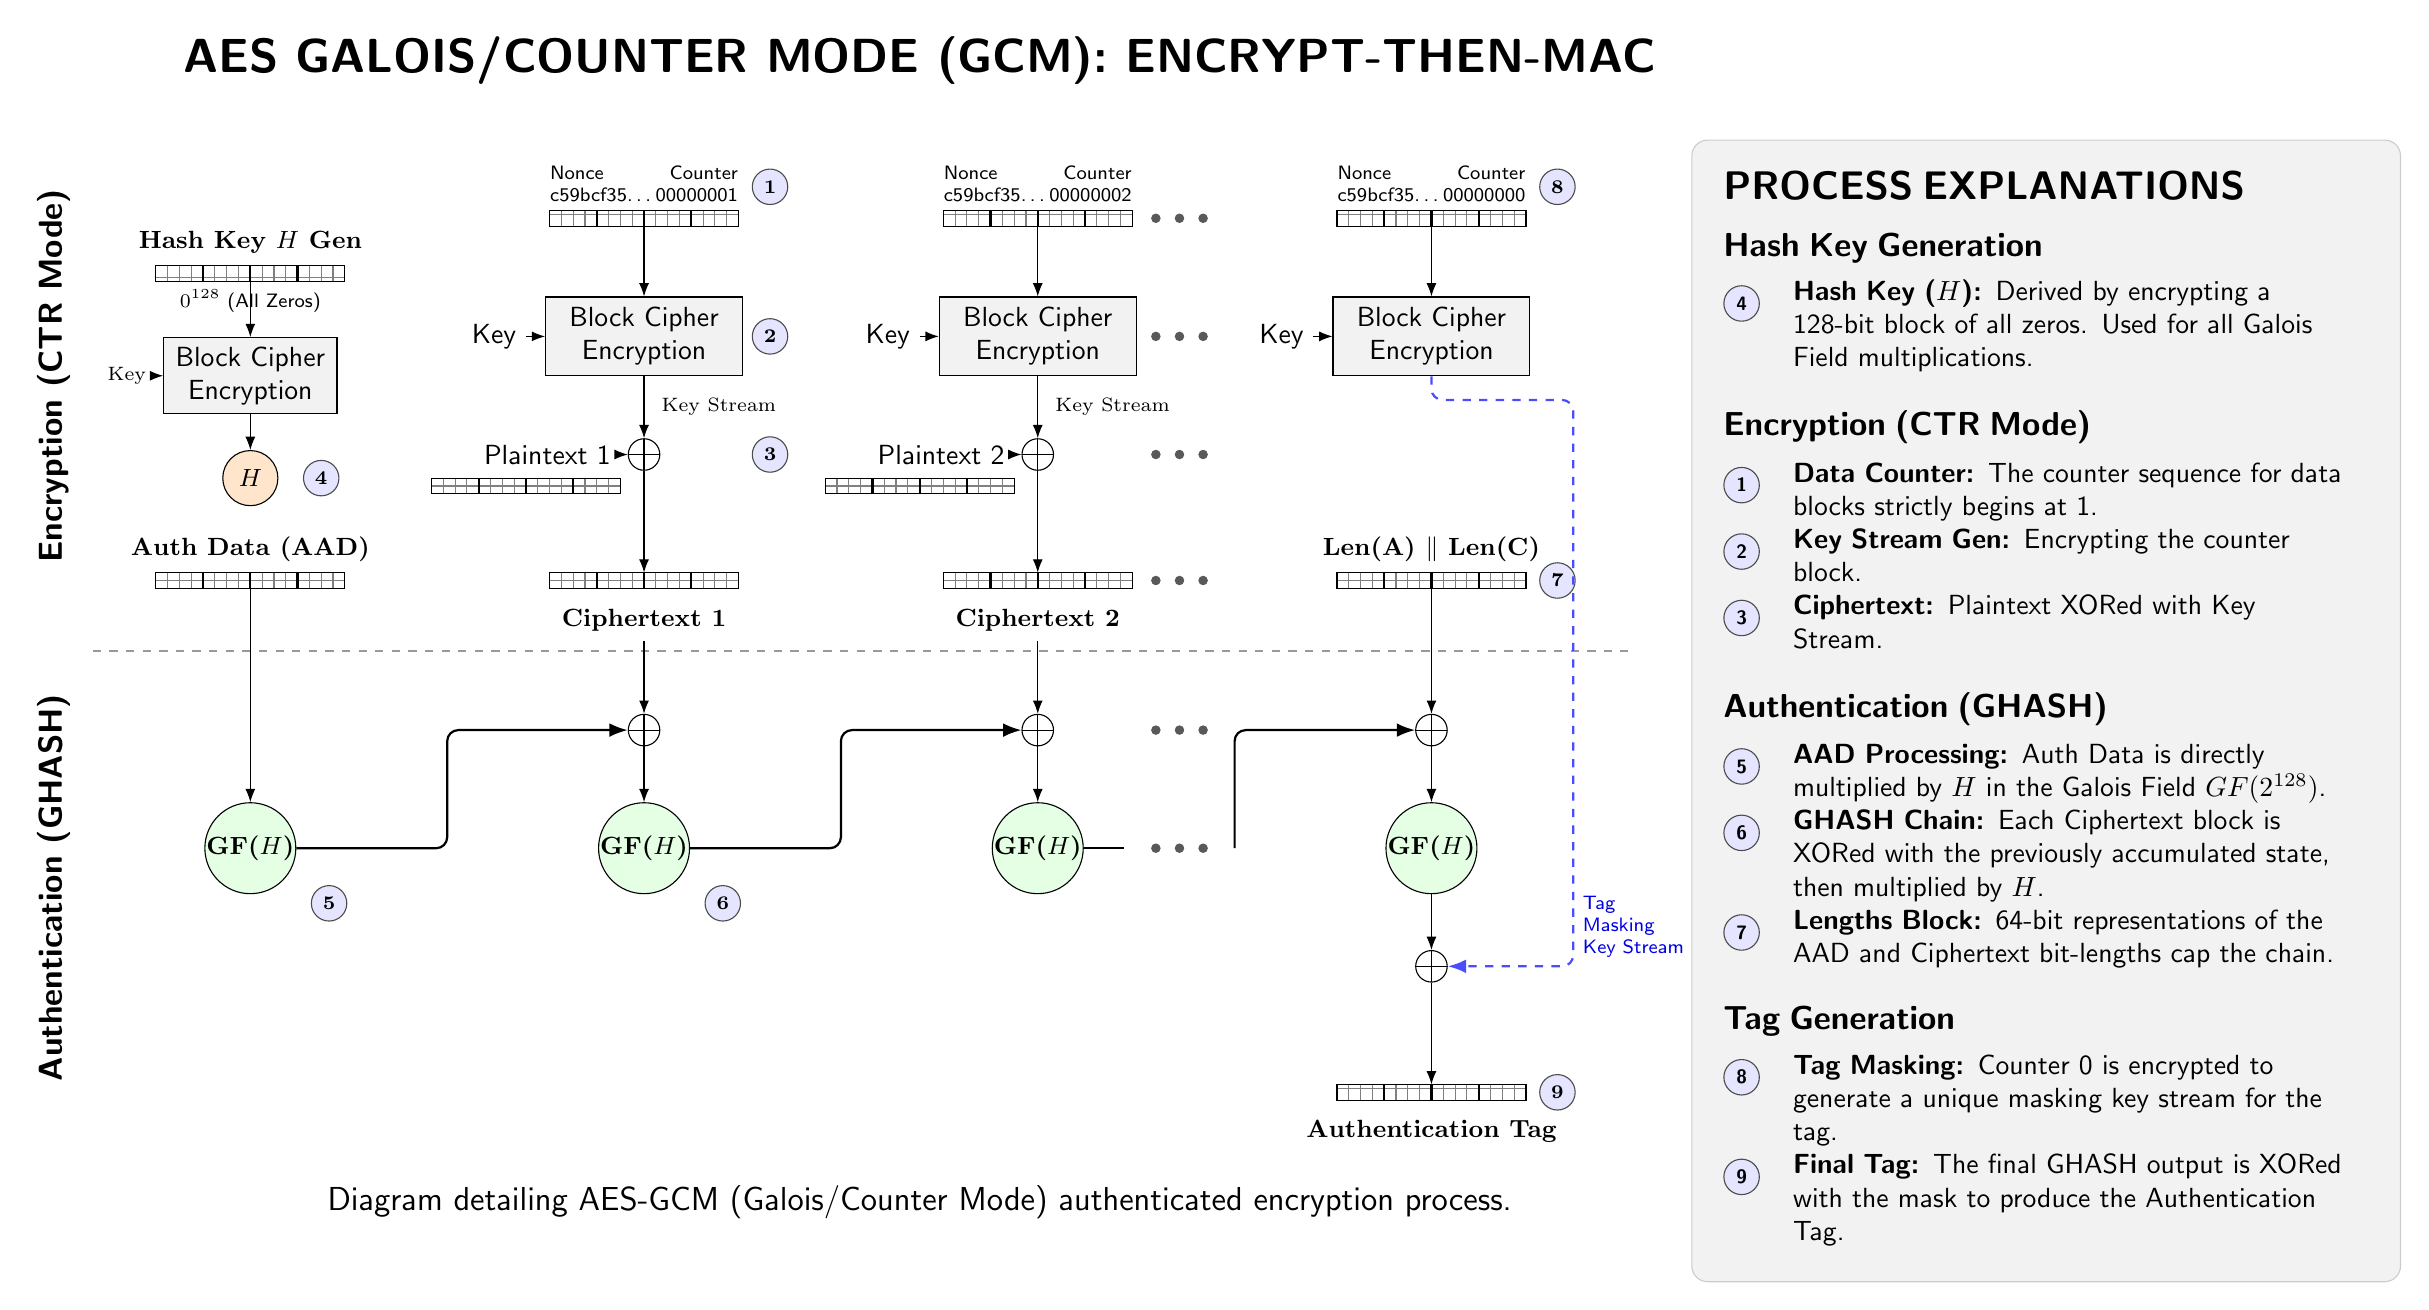
\begin{tikzpicture}[
        >=Latex,
        font=\sffamily,
        cipher/.style={draw, minimum width=2.5cm, minimum height=1cm, align=center, fill=black!5},
        xor/.style={draw, circle, inner sep=0pt, minimum size=0.4cm, path picture={
                        \draw (path picture bounding box.north) -- (path picture bounding box.south)
                        (path picture bounding box.east) -- (path picture bounding box.west);
                    }},
        gf/.style={draw, circle, inner sep=0pt, minimum size=0.9cm, fill=green!10, font=\small\bfseries, align=center},
        indicator/.style={circle, draw=black!70, fill=blue!10, inner sep=0pt, minimum size=4.5mm, font=\scriptsize\bfseries, align=center},
        section title/.style={font=\Large\bfseries\sffamily, anchor=west}
    ]

    % ==========================================
    % TITLES AND SEPARATORS
    % ==========================================
    \node[font=\LARGE\bfseries\sffamily, anchor=center] at (3.5, 6.0) {AES GALOIS/COUNTER MODE (GCM): ENCRYPT-THEN-MAC};
    % Moved the rotated titles further left to x = -7.5 to avoid intersection
    \node[rotate=90, font=\large\bfseries\sffamily] at (-7.5, 2.0) {Encryption (CTR Mode)};
    \node[rotate=90, font=\large\bfseries\sffamily] at (-7.5, -4.5) {Authentication (GHASH)};

    % Dashed line separating Encryption and Authentication (extended left to -7.0)
    \draw[dashed, thick, gray!80] (-7.0, -1.5) -- (12.5, -1.5);


    % ==========================================
    % COLUMN 0: HASH KEY & AAD PROCESSING
    % ==========================================

    % Hash Key H Generation (Top Left)
    \begin{scope}[xshift=-5cm, yshift=2.5cm]
        \node[align=center, font=\small\bfseries] at (0, 1.2) {Hash Key $H$ Gen};

        % Zeros Input
        \draw[gray, thin, step=0.15cm, fill=black!10] (-1.2, 0.7) grid (1.2, 0.9);
        \draw (-1.2, 0.7) rectangle (1.2, 0.9);
        \draw[thick] (-0.6, 0.7) -- (-0.6, 0.9) (0, 0.7) -- (0, 0.9) (0.6, 0.7) -- (0.6, 0.9);
        \node[align=center, font=\scriptsize\sffamily] at (0, 0.45) {$0^{128}$ (All Zeros)};

        % Cipher
        \node[cipher, minimum width=2.2cm, minimum height=0.8cm] (encH) at (0, -0.5) {Block Cipher\\Encryption};
        \draw[->] (0, 0.7) -- (encH);
        \node[anchor=east, font=\scriptsize] (keyH) at (-1.2, -0.5) {Key};
        \draw[->] (keyH) -- (encH);

        % H Output
        \node[gf, fill=orange!20, minimum size=0.7cm] (Hout) at (0, -1.8) {$H$};
        \draw[->] (encH) -- (Hout);
        \node[indicator] at (0.9, -1.8) {4};
    \end{scope}

    % Auth Data (AAD) Processing (Bottom Left)
    \begin{scope}[xshift=-5cm]
        \node[align=center, font=\small\bfseries] at (0, -0.2) {Auth Data (AAD)};

        % AAD Register
        \draw[gray, thin, step=0.15cm, fill=cyan!10] (-1.2, -0.7) grid (1.2, -0.5);
        \draw (-1.2, -0.7) rectangle (1.2, -0.5);
        \draw[thick] (-0.6, -0.7) -- (-0.6, -0.5) (0, -0.7) -- (0, -0.5) (0.6, -0.7) -- (0.6, -0.5);

        % First GF(H) Multiplier
        \node[gf] (gf0) at (0, -4) {GF($H$)};
        % Moved indicator 5 down to avoid horizontal line crossing it
        \node[indicator] at (1.0, -4.7) {5};

        \draw[->] (0, -0.7) -- (gf0.north);
    \end{scope}


    % ==========================================
    % COLUMNS 1 & 2: MAIN DATA BLOCKS
    % ==========================================
    \foreach \i/\ctr/\x in {1/00000001/0, 2/00000002/5} {
            \begin{scope}[xshift=\x cm]

                % Nonce and Counter Labels
                \node[align=left, anchor=south west, inner sep=0, font=\scriptsize\sffamily] at (-1.2, 4.2) {Nonce\\c59bcf35\dots};
                \node[align=right, anchor=south east, inner sep=0, font=\scriptsize\sffamily] at (1.2, 4.2) {Counter\\\ctr};
                \ifnum\i=1 \node[indicator] at (1.6, 4.4) {1}; \fi

                % Counter Register
                \draw[gray, thin, step=0.15cm, fill=gray!20] (-1.2, 3.9) grid (1.2, 4.1);
                \draw (-1.2, 3.9) rectangle (1.2, 4.1);
                \draw[thick] (-0.6, 3.9) -- (-0.6, 4.1) (0, 3.9) -- (0, 4.1) (0.6, 3.9) -- (0.6, 4.1);

                % Block Cipher
                \node[cipher] (enc\i) at (0, 2.5) {Block Cipher\\Encryption};
                \draw[->] (0, 3.9) -- (enc\i);
                \node[anchor=east] (key\i) at (-1.5, 2.5) {Key};
                \draw[->] (key\i) -- (enc\i);
                \ifnum\i=1 \node[indicator] at (1.6, 2.5) {2}; \fi

                % XOR operator and Key Stream Label
                \node[xor] (xorTop\i) at (0, 1) {};
                \draw[->] (enc\i) -- (xorTop\i) node[midway, right, xshift=1mm, font=\scriptsize] {Key Stream};

                % Plaintext Label & Register
                \node[anchor=east] (pt\i) at (-0.3, 1) {Plaintext \i};
                \draw[->] (pt\i) -- (xorTop\i);

                \draw[gray, thin, step=0.15cm] (-2.7, 0.5) grid (-0.3, 0.7);
                \draw (-2.7, 0.5) rectangle (-0.3, 0.7);
                \draw[thick] (-2.1, 0.5) -- (-2.1, 0.7) (-1.5, 0.5) -- (-1.5, 0.7) (-0.9, 0.5) -- (-0.9, 0.7);
                \ifnum\i=1 \node[indicator] at (1.6, 1) {3}; \fi

                % Ciphertext Register & Label
                \draw[gray, thin, step=0.15cm, fill=gray!40] (-1.2, -0.7) grid (1.2, -0.5);
                \draw (-1.2, -0.7) rectangle (1.2, -0.5);
                \draw[thick] (-0.6, -0.7) -- (-0.6, -0.5) (0, -0.7) -- (0, -0.5) (0.6, -0.7) -- (0.6, -0.5);
                \node[align=center, font=\small\bfseries] (ctName\i) at (0, -1.1) {Ciphertext \i};
                \draw[->] (xorTop\i) -- (0, -0.5);

                % GHASH XOR
                \node[xor] (xorBot\i) at (0, -2.5) {};
                \draw[->] (ctName\i.south) -- (xorBot\i.north);

                % GHASH GF(H) Multiplier
                \node[gf] (gf\i) at (0, -4) {GF($H$)};
                \draw[->] (xorBot\i) -- (gf\i);
                % Moved indicator 6 down to avoid horizontal line crossing it
                \ifnum\i=1 \node[indicator] at (1.0, -4.7) {6}; \fi
            \end{scope}
        }


    % ==========================================
    % CONTINUATION DOTS
    % ==========================================
    \foreach \y in {4, 2.5, 1, -0.6, -2.5} {
            \foreach \x in {6.5, 6.8, 7.1} { \filldraw[gray!70!black] (\x, \y) circle (1.5pt); }
        }
    \foreach \x in {6.5, 6.8, 7.1} { \filldraw[gray!70!black] (\x, -4) circle (1.5pt); }


    % ==========================================
    % COLUMN 3: FINALIZATION (TAG & MASK)
    % ==========================================
    \begin{scope}[xshift=10cm]

        % Nonce and Counter 0 (Masking)
        \node[align=left, anchor=south west, inner sep=0, font=\scriptsize\sffamily] at (-1.2, 4.2) {Nonce\\c59bcf35\dots};
        \node[align=right, anchor=south east, inner sep=0, font=\scriptsize\sffamily] at (1.2, 4.2) {Counter\\00000000};
        \node[indicator] at (1.6, 4.4) {8};

        \draw[gray, thin, step=0.15cm, fill=purple!10] (-1.2, 3.9) grid (1.2, 4.1);
        \draw (-1.2, 3.9) rectangle (1.2, 4.1);
        \draw[thick] (-0.6, 3.9) -- (-0.6, 4.1) (0, 3.9) -- (0, 4.1) (0.6, 3.9) -- (0.6, 4.1);

        % Mask Encryption
        \node[cipher] (enc3) at (0, 2.5) {Block Cipher\\Encryption};
        \draw[->] (0, 3.9) -- (enc3);
        \node[anchor=east] (key3) at (-1.5, 2.5) {Key};
        \draw[->] (key3) -- (enc3);

        % Lengths Register
        \node[align=center, font=\small\bfseries] at (0, -0.2) {Len(A) $\parallel$ Len(C)};
        \draw[gray, thin, step=0.15cm, fill=yellow!20] (-1.2, -0.7) grid (1.2, -0.5);
        \draw (-1.2, -0.7) rectangle (1.2, -0.5);
        \draw[thick] (-0.6, -0.7) -- (-0.6, -0.5) (0, -0.7) -- (0, -0.5) (0.6, -0.7) -- (0.6, -0.5);
        \node[indicator] at (1.6, -0.6) {7};

        % Lengths XOR
        \node[xor] (xorBot3) at (0, -2.5) {};
        \draw[->] (0, -0.7) -- (xorBot3.north);

        % Final GF(H) Multiplier
        \node[gf] (gf3) at (0, -4) {GF($H$)};
        \draw[->] (xorBot3) -- (gf3);

        % Final Tag XOR (Combines GHASH output with Tag Mask)
        \node[xor] (xorFinal) at (0, -5.5) {};
        \draw[->] (gf3) -- (xorFinal);

        % Authentication Tag Output Register
        \draw[gray, thin, step=0.15cm, fill=red!20] (-1.2, -7.2) grid (1.2, -7.0);
        \draw (-1.2, -7.2) rectangle (1.2, -7.0);
        \draw[thick] (-0.6, -7.2) -- (-0.6, -7.0) (0, -7.2) -- (0, -7.0) (0.6, -7.2) -- (0.6, -7.0);
        \node[align=center, font=\small\bfseries] at (0, -7.6) {Authentication Tag};
        \draw[->] (xorFinal) -- (0, -7.0);
        \node[indicator] at (1.6, -7.1) {9};
    \end{scope}


    % ==========================================
    % ROUTING & CONNECTIONS
    % ==========================================

    \draw[->, rounded corners, thick] (gf0.east) -- (-2.5, -4) -- (-2.5, -2.5) -- (xorBot1.west);
    \draw[->, rounded corners, thick] (gf1.east) -- (2.5, -4) -- (2.5, -2.5) -- (xorBot2.west);
    \draw[-, rounded corners, thick] (gf2.east) -- (6.1, -4);

    \draw[->, rounded corners, thick] (7.5, -4) -- (7.5, -2.5) -- (xorBot3.west);

    \draw[->, rounded corners, thick, dashed, blue!70]
    (enc3.south) -- ++(0, -0.3) -| (11.8, -5.5) -- (xorFinal.east);
    \node[right, align=left, font=\scriptsize\sffamily, text=blue!90!black] at (11.8, -5.0) {Tag\\Masking\\Key Stream};


    % ==========================================
    % EXPLANATORY SIDE PANEL
    % ==========================================
    \node[anchor=north west, fill=black!5, draw=black!20, rounded corners=2mm, inner sep=4mm, text width=8.2cm, align=left] at (13.3, 5.0) {
        \textbf{\Large PROCESS EXPLANATIONS}\\[3mm]

        \textbf{\large Hash Key Generation}\\[1.5mm]
        \begin{tabular}{@{}c >{\raggedright\arraybackslash}p{7.0cm}@{}}
            \tikz[baseline=-0.8ex]{\node[indicator]{4};} & \textbf{Hash Key ($H$):} Derived by encrypting a 128-bit block of all zeros. Used for all Galois Field multiplications.
        \end{tabular}\\[4mm]

        \textbf{\large Encryption (CTR Mode)}\\[1.5mm]
        \begin{tabular}{@{}c >{\raggedright\arraybackslash}p{7.0cm}@{}}
            \tikz[baseline=-0.8ex]{\node[indicator]{1};} & \textbf{Data Counter:} The counter sequence for data blocks strictly begins at 1. \\[1.5mm]
            \tikz[baseline=-0.8ex]{\node[indicator]{2};} & \textbf{Key Stream Gen:} Encrypting the counter block.                            \\[1.5mm]
            \tikz[baseline=-0.8ex]{\node[indicator]{3};} & \textbf{Ciphertext:} Plaintext XORed with Key Stream.
        \end{tabular}\\[4mm]

        \textbf{\large Authentication (GHASH)}\\[1.5mm]
        \begin{tabular}{@{}c >{\raggedright\arraybackslash}p{7.0cm}@{}}
            \tikz[baseline=-0.8ex]{\node[indicator]{5};} & \textbf{AAD Processing:} Auth Data is directly multiplied by $H$ in the Galois Field $GF(2^{128})$.                 \\[1.5mm]
            \tikz[baseline=-0.8ex]{\node[indicator]{6};} & \textbf{GHASH Chain:} Each Ciphertext block is XORed with the previously accumulated state, then multiplied by $H$. \\[1.5mm]
            \tikz[baseline=-0.8ex]{\node[indicator]{7};} & \textbf{Lengths Block:} 64-bit representations of the AAD and Ciphertext bit-lengths cap the chain.
        \end{tabular}\\[4mm]

        \textbf{\large Tag Generation}\\[1.5mm]
        \begin{tabular}{@{}c >{\raggedright\arraybackslash}p{7.0cm}@{}}
            \tikz[baseline=-0.8ex]{\node[indicator]{8};} & \textbf{Tag Masking:} Counter 0 is encrypted to generate a unique masking key stream for the tag.    \\[1.5mm]
            \tikz[baseline=-0.8ex]{\node[indicator]{9};} & \textbf{Final Tag:} The final GHASH output is XORed with the mask to produce the Authentication Tag.
        \end{tabular}
    };

    % Bottom Caption
    \node[font=\large\sffamily, anchor=center] at (3.5, -8.5) {Diagram detailing AES-GCM (Galois/Counter Mode) authenticated encryption process.};

\end{tikzpicture}
\end{document}